Let $\module{F}$ be a quasi-coherent module on $\overcat{C}{a}$.
We have to show that $\sections{a}{F} \tensor_{\sections{a}{O}} \sections{b}{O} \xrightarrow{k} \sections{b}{F}$ is an isomorphism. 
The map $k$ is the adjunct of $\module{F}(f)$ with respect to the adjunction between restricting scalars and extending scalars along the map 
$\sections{a}{O} \rightarrow \sections{b}{O}$. 
More concretely, this map is

\[k: x \tensor m \mapsto \module{F}(f)(x)m.\]

The argument will go as follows. 
First we observe that the morphism $\counit_{\module{F}}:\module{F} \rightarrow \Tildefunctor{\globalsections{F}}$ is an isomorphism because $a$ is caffine.
Second $i_{a}:\Kappa{\globalsections{F}}(a) \rightarrow \Tildefunctor{\globalsections{F}}(a)$ is an isomorphism by lemma .. . 
This holds for any caffine objects, so also for $b$. 
The consequence is that $\Kappa{\globalsections{F}}(f) = i_b^{-1} \module{F}(f) \circ i_a$, by naturality of the transformation 
$i: \Kappa{\globalsections{F}}\rightarrow \module{F}$.
Third, show that $\Kappa{\globalsections{F}}(f)$ has an isomorphism as adjunct along the same extension/restriction adjunction. Call this adjunct $k'$.
Fourth, use naturality of adjunction bijections to conclude that $k$ must also be an isomorphism.

Since $a$ is caffine, $\module{F} = \Tildefunctor{\globalsections{F}}$.
Since $\Tildefunctor{\blank} = \sheafify{\blank} \circ \Kappa{\blank}$, we know that $\module{F}$ is the sheafification of the presheaf 
\[\Kappa{\globalsections{F}} = c \rightarrow \sections{a}{F} \tensor_{\sections{a}{O}} \sections{c}{O}.\]
Set $M = \sections{a}{F}$.

Define $k': \sections{a}{\Kappa{M}} \tensor_{\sections{a}{O}} \sections{b}{O} \rightarrow \sections{b}{\Kappa{M}}$
By $k':x \tensor m \mapsto \Kappa{M}(f)(x) m$.
If you unfold the constructions, it follows that 
\[k'(x\tensor m) = x\tensor m \in \sections{b}{\Kappa{M}} = M \tensor \sections{b}{O}\]
 is actually the identity.

We will prove that $
A) The component at a caffine object of the unversal sheafification morphism $i$ is an isomorphism
As is stated in lemma .. , we have $\globalsections{i} = \counit_{T,a}$. 
Hence when $a$ is caffine then $\globalsections{i}$ on is an iso.
Note that $\globalsections{i}:\cat{C}/x \rightarrow \modules{\sheaf{O}(x)}$ is equal to $\sections{x}{i}: \cat{C}{y} \rightarrow \

%By naturality of the universal sheafification transformation $i$, $\sections{a}{i}$ is an iso for all caffine $a$. 


B) Adjunction bijection respects composition with isos
We have now that $\Kappa{M}(f) = i_b^{-1} \circ \Tildefunctor{F}(f) \circ i_a$. Let $F$ be the bijection from the adjunction $\mainadjunction$.
Then $

C) Hence $k$ is also an iso.



Note that restricting and sheafification commute.%TODO: explain
We can first restrict our presheaf to $\cat{C}/b$ and then sheafify. 
The global sections component of the universal sheafification morphism will be 
\[M \tensor \sections{b}{O} \rightarrow \sections{b}{F},\]
\[m \tensor r \mapsto mr\]

because the triangle 

\begin{center}
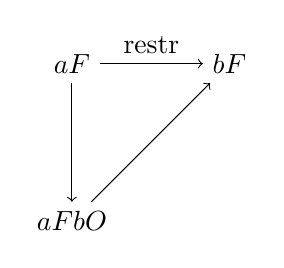
\begin{tikzpicture}[node distance=2cm, auto]
  \node (C) {$\sections{a}{F}$};
  \node (B) [right of =C] {$\sections{b}{F}$};
  \node (D) [below of= C]{$\sections{a}{F}\tensor \sections{b}{O}$};
  \draw[->] (C) to node {$\mbox{restr}$} (B);
  \draw[->] (D) to node [swap] {}  (B);
  \draw[->] (C) to node [swap] {} (D);
\end{tikzpicture}
\end{center}

must commute by naturality. This is exactly the component of the unit $\eta$ of the $\mainadjunction$ on $\site{C}{T}{O}/b$ for $\sections{a}{F} \tensor \sections{b}{O}$.
Since $b$ is caffine, this is an isomorphism by assumption.

Let $\ringedsite{C}{T}{O}$ be a ringed site.
Let $R=\globalsections{O}$. Let $a\in C$ and $f:x\rightarrow y \in C$.